% This is samplepaper.tex, a sample chapter demonstrating the
% LLNCS macro package for Springer Computer Science proceedings;
% Version 2.20 of 2017/10/04
%
\RequirePackage{fix-cm}
\documentclass[runningheads]{llncs}
%
\usepackage{graphicx}
\usepackage[utf8x]{inputenc}
\usepackage[T1]{fontenc}
\usepackage{subcaption}
\usepackage{qtree}
\usepackage{booktabs}
\usepackage{fancybox}
\usepackage[export]{adjustbox}
\usepackage{pgfplots}
\usepackage{pgfplotstable}
\usepackage{placeins}
\usepackage{dblfloatfix}
\usepackage{amsbsy}
\usepackage{tikz}
\usetikzlibrary{positioning}

% Used for displaying a sample figure. If possible, figure files should
% be included in EPS format.
%
% If you use the hyperref package, please uncomment the following line
% to display URLs in blue roman font according to Springer's eBook style:
% \renewcommand\UrlFont{\color{blue}\rmfamily}

\newcommand\red[1]{{\color{red}#1}} 
\newcommand\blue[1]{{\color{blue}#1}}

\begin{document}
%
\title{Comparison of tree based strategies for parallel simulation of self-gravity in agglomerates}
%
\titlerunning{Comparison of tree based strategies for self-gravity in agglomerates}
% If the paper title is too long for the running head, you can set
% an abbreviated paper title here
%
\author{Nestor Rocchetti\inst{1} \and
Sergio Nesmachnow\inst{1} \and
Gonzalo Tancredi\inst{2}}
%
\authorrunning{N. Rocchetti, S. Nesmachnow, G. Tancredi}

\institute{Facultad de Ingenier\'ia, Universidad de la Rep\'ublica, Montevideo, Uruguay \email{\{nrocchetti,sergion\}@fing.edu.uy}\\ \and
Facultad de Ciencias, Universidad de la Rep\'ublica, Montevideo, Uruguay \email{gonzalo@fisica.edu.uy}}
%
\maketitle              % typeset the header of the contribution
%
\begin{abstract}
This article presents an algorithm conceived to improve the computational efficiency of simulations in ESyS-Particle  that involve a large number of particles. ESyS-Particle applies the Discrete Element Method to simulate the interaction of agglomerates of particles. The proposed algorithm is based on the Barnes \& Hut method, in which a domain is divided and organized in an octal tree. The algorithm is compared to a variation o f the octal tree version that uses a binary tree instead. Experimental evaluation is performed over two scenarios: a collapsing cube scenario and two agglomerates orbiting each other. The experimental evaluation comprises the performance analysis of the two scenarios using the two algorithms, including a comparison of the results obtained and the analysis of the numerical accuracy. Results indicate that the octal tree version performs faster and is more accurate than the binary tree version. 

\keywords{Multithreading, self-gravity, DEM}
\end{abstract}
%
%
%
\section{Introduction}
N-Body simulations are powerful tools for research on astrophysical objects, especially for asteroids and comets composed of agglomerates of particles. In these simulations, particles are affected by short range and long range interactions. Self-gravity~\cite{harris2009shapes,fujiwara2006rubble} is a type of long range interaction that can cause attraction and deformation (tidal disruption) of agglomerates of particles~\cite{walsh2012spin,goldreich2009tidal,rozitis2014cohesive}. A straightforward approach in the process of calculating the acceleration of one particle due to long range interactions in numerical simulations, is to perform the calculation of $N - 1$ forces, one for each of the other particles that compose the system. However, this approach does not scale, as the computational cost of calculating the acceleration for all particles in the system grows quadratically with the number of particles (the algorithm is $O(N^2)$).
 
High Performance Computing (HPC) is a paradigm that proposes the use of multiple computing resources simultaneously. This way, complex problems that demand large computer power can be solved in reasonable execution times. Also, HPC allows to scale problems to larger domains. 

Discrete Element Method (DEM) is a numerical method that comprises contact detection and contact interaction of bodies \cite{cundall1979discrete}. The use of DEM allows performing simulations of millions of particles that can break, fracture, or fragment. The method consists of maintaining a list of near-neighbors for each particle, which is updated periodically. In order to reduce the execution time, knowing which particles are in contact with a given particle consists of checking the neighbor list instead of the complete list of particles. Nonetheless, DEM has a heavy computational cost when performing simulations that comprise millions of particles, when compared to other numerical methods. 

The DEM method is implemented in ESyS-Particle~\cite{abe2009esys}, an open source software for simulation of particle systems that is implemented using parallel programming techniques and is adapted to run in parallel and distributed computing environments. ESyS-Particle does not have a model to simulate long range forces. Our previous works proposed a self gravity implementation module in which HPC techniques were applied to allow simulations comprising thousands of particles~\cite{frascarelli2014high}. Then ~\cite{nesmachnow2015parallel}, strategies were presented for an efficient parallel algorithm for self gravity computation. In addition, the module was integrated in ESyS-Particle and specific performance improvements were implemented, including a method that updates only the occupied cells of a mesh~\cite{rocchetti2017performance}. Later~\cite{rocchetti2018}, strategies based on the Barnes \& Hut octal tree method were implemented and compared to the previously presented occupied cells method.

In this line of work, this article presents a performance comparison of two tree-based methods: a Barnes \& Hut octal tree method~\cite{rocchetti2018}, and a Barnes \& Hut binary tree method. The experimental evaluation comprises the performance analysis of the proposed methods using a standard benchmark scenario for astronomical simulation that consists of two agglomerates orbiting each other. The analysis includes a comparison of the performance results obtained using different number of computing resources (threads) and also the study of the numerical accuracy. The scenario was evaluated using different number of particles and scaling the computational resources. The main scientific contributions included in this article are: i) a Barnes \& Hut binary tree method, ii) an experimental evaluation of the two orbiting agglomerates scenario, and iii) a performance comparison of the Barnes \& Hut octal tree method and the Barnes \& Hut binary tree method.

The article is organized as follows. Section \ref{sec:related_work} reviews the related work on domain decomposition for particle simulations and the previous work by our research group. Section \ref{sec:byh} explains the Barnes \& Hut octal tree implementation evaluated. Section \ref{sec:bin_byh} explains the characteristics of the binary tree implementation and how it was developed using the octal tree as a baseline implementation. Section \ref{sec:test_scenarios} describes the test scenario, the instances created from it, and the computational infrastructure used in the performance comparison. Section \ref{sec:perf_res} reports the main results of the performance evaluation and a discussion on the results obtained. Finally, section \ref{sec:conclusion} presents the conclusions and formulates the main lines for future work. 

\section{Related work: static and dynamic spatial domain decomposition}
\label{sec:related_work}

This section describes the work related to spatial domain decomposition techniques used to speed up the calculation of the long range interactions.

Spatial domain decomposition techniques are classified in static and dynamic. The main difference between those two approaches is that the structures created using a static domain decomposition remain invariant during a simulation, while in dynamic strategies they do not. Hockney and Eastwood~\cite{hockney1988computer} classified static techniques in three models: Particle-Particle (PP) methods, Particle-Mesh (PM) methods, and Particle-Particle Particle-Mesh (P3M) methods. PP is a straightforward method in which the acceleration is calculated considering the individual effect of every particle in the system. Thus, the execution time of PP is $O(n^2)$. PM methods \cite{darden1993particle,essmann1995smooth,sanchez2012simulation,kravtsov1997adaptive} use a mesh of point particles that lies over the spatial domain. The acceleration is computed for point particles and then is propagated to individual particles using interpolation. PM methods are faster that PP methods, but are less accurate. Finally, P3M \cite{couchman1991mesh,macfarland1998new,harnois2013high,brieu1994cosmological} methods combine PP methods (to compute short range forces) and PM methods (to compute long range forces). P3M has proven to be fast and accurate methods to calculate particle forces.

%Spatial dynamic domain decomposition techniques are based on structures that are updated or reconstructed from scratch during a simulation. 
Structures in spatial dynamic domain decomposition techniques are updated or reconstructed from scratch during a simulation. 
The process that updates or reconstructs the structures is triggered by the movement of the particles. Barnes and Hut~\cite{barnes1986hierarchical} proposed a technique that uses an octal tree to represent the spatial domain of a simulation. Results showed that the calculation time of the long range interactions is of $O(N log N)$, being $N$ the number of particles in the system. Greengard and Rokhlin~\cite{greengard1987fast} presented the Fast Multipole Method (FMM), another dynamic domain decomposition method. FMM implements a multipole expansions on the system that are organized as a hierarchy of meshes. Results presented by Greengard and Rokhlin indicate that the performance of FMM is $300\times$ faster than the PP method.

Techniques that combine static and dynamic domain decomposition techniques are present in the literature. Xu \cite{xu1994new} presented the Tree Particle Mesh (TPM) method. In TPM, short range interactions are calculated using tree methods, while long range interactions are calculated using the PM method. Reported results indicated that TPM is $12\times$ faster than using only a tree method. Bode et al.~\cite{bode2000tree} presented a TPM implementation in which the trees are updated individually. According to the authors, their TPM implementation speeds up the simulations ``by a factor of three or four" compared to the P3M method. Bagla \cite{bagla2002treepm} presented the TreePM method, in which the short range forces are calculated using the Barnes and Hut tree code, while the long range forces are calculated using the PM code. Results presented by Bagla show that the TreePM method is $4.5\times$ faster than a tree code. Then, Khandai and Bagla \cite{khandai2009modified} presented a modification of the TreePM where the particles are associated to groups. Particles are grouped based on the particle count per unit of volume. According to Khandai and Bagle, the proposed modified TreePM is $12.72\times$ faster than the TreePM without modifications.   

Previous work performed by our group includes the proposal of a hierarchical grouping approximation method called Mass Approximation Distance Algorithm (MADA) by Frascarelli et al.~\cite{frascarelli2014high}. MADA is a specialization of the P3M method that allowed improving the performance of calculating the acceleration of particles by considering groups of distant particles as a single point particle. After that, Nesmachnow et al.~\cite{nesmachnow2015parallel} presented, analyzed and compared data-assignment patterns for self-gravity calculation using MADA. Results showed that the best of the proposed patterns was the Advanced Isolated Linear strategy. In this strategy, workload is assigned equally to all the threads available. Then, whenever a thread finishes working, unprocessed workload is reassigned to it. 
%According to the authors, 
The speedup was close to linear in tests performed for systems with up to $2$$\times$$10^5$ particles. Rocchetti et al.~\cite{rocchetti2017performance} implemented the algorithm for calculating self-gravity in ESyS-Particle. A performance analysis and an improved implementation of the algorithm in which the acceleration is recalculated only for the occupied cells of the system was introduced. Results showed a speedup of $50\times$ of the improved version compared to the baseline (non optimized) version. 

\section{Implementation of the Barnes \& Hut tree}
\label{sec:byh}
This section explains the characteristics of the Barnes \& Hut tree implemented for the self-gravity calculation in ESyS-Particle. Then, the process of creation of the tree and self-gravity calculation is shown.

\subsection{Octal tree structure}
The Barnes \& Hut tree is implemented as an octal tree in which the root represents the complete space used for the simulation. Leaf nodes of the tree are the boxes of the self-gravity grid. Every non-leaf node has eight sons that have the same size. So, the space represented by the tree is of cubical shape. Each node also has the following information: the position of the center of mass, the total mass, the spatial coordinates, the coordinates in the self-gravity grid, the level number,the number of particles in it, and an integer that identifies the node in the level it belongs. All nodes of a level are numbered from $0$ to $n-1$ being $n$ the number of nodes of the level. The identifiers are assigned to the nodes so that the id of the father of a node satisfies that $id_f=id_s/(10_8 \times (level_s / level_f)$, where $id_x$ is the identifier of the node, and $level_x$ is the level of the node. The underscore `8' denotes that the number is in octal base. This way, to know if a node is son of another is an constant time operation performed in $O(1)$. Dividing by $10_8$ the identifier of a node is equivalent to performing a shift operation of three bits to the right. Figure \ref{fig:pelota} shows a sample two-dimensional tree partition created for an agglomerates of particles. The resolution of the partition is not increased on the nodes that have no particles by stating that the tree node created is empty after its creation. 

\begin{figure}[!h]
\setlength{\abovecaptionskip}{3pt}
   	\centering
	\includegraphics[ trim = 0mm 0mm 56.5mm 56.5mm, clip, width=0.40\textwidth]{pelota.png}
	\caption{Example of tree partition created for an agglomerate of particles. The example is represented as a two dimensions projection)}
	\label{fig:pelota}
\end{figure}

\subsection{Creating the tree}

The tree is created by level, from the root node to the leaf nodes. In this step, the identifier of the nodes is assigned. The root node, that represents the whole (cubic) space, is divided into cubes of equal size. This operation is performed recursively for each level of the tree that is spawned. The creation of new levels ends when the size of the nodes matches the size of the grid boxes.  
After the creation of the tree, the centers of mass of the nodes are calculated. The process of calculation of the centers of mass is bottom up, from the leaves up to the root node. The centers of mass for the leaf nodes are calculated directly from the particles, whereas for the nodes of the upper levels the centers of mass are calculated from their respective son nodes. The center of mass is calculated only for the nodes that have particles. Figure \ref{fig:arb_octal} shows a sample octal tree created using the algorithm described for a cube composed of 64 boxes. As an example, the center of mass for the node in the upper left of the figure will not be calculated because it has no particles.  

\begin{figure}[!h]
\setlength{\abovecaptionskip}{3pt}
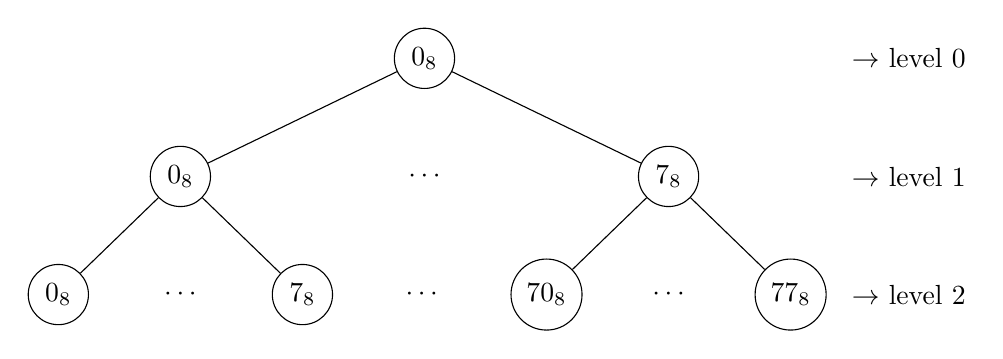
\begin{tikzpicture}[level/.style={sibling distance=31mm/#1}]
\node [circle,draw] (z){$0_8$}
  child {node [circle,draw] (a) {$0_8$}
    child {node [circle,draw] (b) {$0_8$}}
    child {node {$\cdots$} edge from parent[draw=none]} 
    child {node [circle,draw] (g) {$7_8$}}
  }
  child {node {$\cdots$} edge from parent[draw=none]}
  child {node [circle,draw] (j) {$7_8$}
    child {node [circle,draw] (k) {$70_8$}}
    child {node {$\cdots$} edge from parent[draw=none]}
  child {node [circle,draw] (l) {$77_8$}   
        child [grow=right] {node (s) {$\rightarrow$ level 2} edge from parent[draw=none]
             child [grow=up] {node (t) {$\rightarrow$ level 1} edge from parent[draw=none]
                 child [grow=up] {node (u) {$\rightarrow$ level 0} edge from parent[draw=none]}
          }
        }       
        }
};
\path (g) -- (k) node [midway] {$\cdots$};
\end{tikzpicture}

	\caption{Example of numeration for a three level octal tree for a self-gravity grid composed of 64 boxes.}
	\label{fig:arb_octal}
\end{figure}

\subsection{Updating self-gravity}

Once the tree is created and the centers of mass are calculated, the \textit{list of tree nodes} is built for each of the occupied boxes of the self-gravity grid (called \textit{objective nodes}) by using the tree as input data. A part of the list is composed of the \textit{neighbor nodes} of the objective node. The \textit{neighborhood} is defined as those boxes that are located less than a certain distance, measured in number of boxes, from the objective node. The threshold distance is set as a parameter of the algorithm. The rest of the list is composed of the highest level nodes contain particles and that are not father of any member of the neighborhood. For example, defining a neighborhood of size 0 and assuming that all the cells are occupied, the list of nodes for node $77_8$ for the tree of figure \ref{fig:arb_octal} is composed of nodes $0_8$ to $6_8$ of level 1 and $70_8$ to $76_8$ of level 2. The root node is never a part of the list of nodes because it is the father of all nodes, since as it represents the complete space of a scenario.

After creating the list of nodes for all the nodes in the occupied boxes list, the potential of each node is calculated in parallel using threads. Afterwards, the results are communicated to the particle module, the tree is destroyed, and its memory freed.  

\section{Implementation of the binary tree}
\label{sec:bin_byh}

This section presents the binary tree. The changes introduced in the octal tree algorithm to implement it the binary tree and the main differences between both implementations are described. 

\subsection{Structure and process of creation of the binary tree}

Figure \ref{fig:arb_bin} shows a sample binary tree for a self-gravity grid composed of 64 boxes. The generated tree has seven levels, including the root level. Each node has a unique number that identifies it in the corresponding level, which is an integer in binary code. A node is the father of another node of the binary tree if it satisfies that $id_f=id_s/(10_2 \times (level_s / level_f)$, where $id_x$ is the identifier of the node and $level_x$ is the level of the node. The underscore 2 denotes that the number is in binary base. This way, to know if a node is son of another is an operation of $O(1)$. This condition is the same used to the octal tree but modified to check the condition in binary base. Instead of dividing by $10_8$, the division is performed by $10_2$ which comprises a shift operation to the right. 

\begin{figure}[!h]
\setlength{\abovecaptionskip}{3pt}
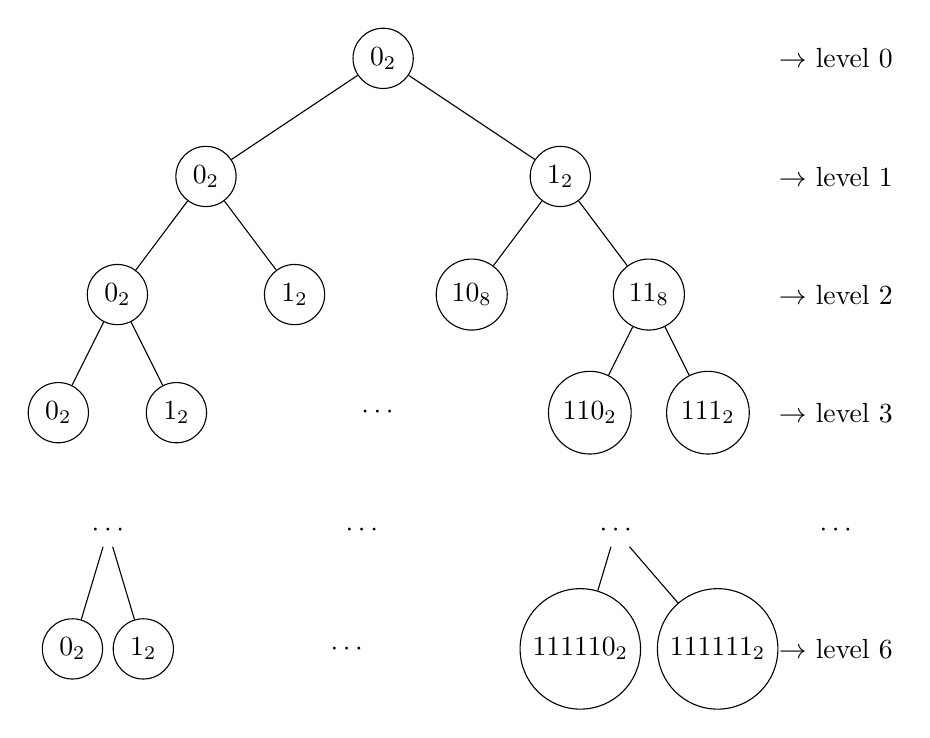
\begin{tikzpicture}[level/.style={sibling distance=45mm/#1}]
\node [circle,draw] (z){$0_2$}
  child {node [circle,draw] (a) {$0_2$}
    child {node [circle,draw] (b) {$0_2$}
    	child {node [circle,draw] (c) {$0_2$}
        	child {node (cc) [right=0.3cm] {$\cdots$} edge from parent[draw=none]
            	child {node [circle,draw] (l) {$0_2$}}
        		child {node [circle,draw] (m) {$1_2$}}
            }
        }
        child {node [circle,draw] (d) {$1_2$}}
    }
    child {node [circle,draw] (g) {$1_2$}}
  }
  child {node [circle,draw] (j) {$1_2$}
    child {node [circle,draw] (k) {$10_8$}}
  child {node [circle,draw] (l) {$11_8$}
  		child {node [circle,draw] (e) {$110_2$}}
        child {node [circle,draw] (f) {$111_2$}
        	child {node (ff) [right=-1.5cm] {$\cdots$} edge from parent[draw=none]
                	child {node [circle,draw] (fffe) {$111110_2$}}
        			child {node [circle,draw] (ffff) [right=0.2cm of fffe] {$111111_2$}
        child [grow=right] {node (w) {$\rightarrow$ level 6} edge from parent[draw=none]
        child [grow=up] {node (v) {$\cdots$} edge from parent[draw=none]
        child [grow=up] {node (v) {$\rightarrow$ level 3} edge from parent[draw=none]
        child [grow=up] {node (s) {$\rightarrow$ level 2} edge from parent[draw=none]
             child [grow=up] {node (t) {$\rightarrow$ level 1} edge from parent[draw=none]
                 child [grow=up] {node (u) {$\rightarrow$ level 0} edge from parent[draw=none]}         	     
                }
              }
            }
            }
            }
          }
          }
        }       
      }
};
\path (d) -- (e) node [midway] {$\cdots$};
\path (m) -- (fffe) node [midway] {$\cdots$};
\path (cc) -- (ff) node [midway] {$\cdots$};
\end{tikzpicture}
	\caption{Example of enumeration for a binary tree with seven levels for a self-gravity grid composed of 64 boxes.}
	\label{fig:arb_bin}
\end{figure}

To build the tree, the space represented by a node is divided in two by its largest edge. So, the partitions are not necessarily cubic. This way, the binary tree has the advantage that the space represented does not need to be cubic. Performing the partitions over the largest edge guarantees that the leaf nodes are of the same size and position of the self-gravity grid boxes. 

\subsection{Comparison of the binary tree and the octal tree}

The node used for the octal tree example in Figure \ref{fig:arb_octal} is $77_8$, which corresponds to $111111_2$ in the binary tree. Assuming that all the boxes are occupied and the neighborhood size is zero, in the binary tree in Figure \ref{fig:arb_bin} the list of tree nodes is comprised of node $0_2$ (level 1), node $10_2$ (level 2), node $110_2$ (level 3), node $1110_2$ (level 4), and node $11110_2$ (level 5). In this example, the list of tree nodes has five elements. On the other hand, the list of tree nodes of the octal tree has 13 elements. Despite having more levels, the list of tree nodes for the binary tree has fewer elements then the octal tree 
%In addition, 
and
the resolution of the partition for the binary tree grows slower when moving closer to the objective node.   

Except for the aforementioned differences, 
%the rest of 
the structure is the same as the octal tree. The algorithm to update self-gravity in the binary tree is the same as the octal tree. After creating the lists of nodes for the occupied nodes, the gravitational potential is calculated and handled to the ESyS-particle module.  
 
\section{Experimental evaluation setup}
\label{sec:test_scenarios}

This section describes the test scenario and the different instances used to perform the experimental evaluation of the proposed tree-based methods for self-gravity calculation. In addition, characteristics inherent to the simulation and the infrastructure used to perform the simulations are described.

\subsection{Test scenarios}
The scenario used for the performance test is the two agglomerate scenario previously used in Rocchetti et al.~\cite{rocchetti2017performance}. The scenario consists of two agglomerates of particles that are symmetrical with respect to the origin of the coordinates system (point (0,0,0)). This way, the center of mass is located in the point (0,0,0) as well, and it is halfway the center of mass of each agglomerate. Figure \ref{fig:2aglo} shows a two dimensional projection of the two agglomerate scenario. The agglomerates have a diameter of one kilometer and are separated from one another by five kilometers. The extension of the scenario goes from $-4096m$ to $4096m$ over the three dimensions. This way, the resulting scenario is a cube with edges of 8192m. The scenario was created using Gengeo, a package included in ESyS-Particle. In particular, Gengeo was used to create one of the agglomerates and pack it with particles of diverse diameters within a predefined range of sizes. 

Three instances of the two agglomerate scenario were created with different number of particles by varying the minimum and maximum diameter of the particles when using Gengeo. The scenarios were named small, medium, and large, according to the number of particles they have. The small scenario is composed of 3,866 particles with a radius in the range of 50m to 100m. The medium scenario has 11,100 particles with a radius that varies from 35m to 70m. Finally, the large scenario has 38,358 particles which radius varies from 20m to 60m. In all cases, the initial speed of the scenario was configured to be 5m/s in a direction that is tangential to the $z$ axis and perpendicular to the line that passes through the center of mass of each agglomerate. In addition, the total mass of the instances oscillates from $1.2\times10^12 kg$ to $1.7\times10^12 kg$. Also, the density of the particles is $3000 g/cm^3$, a density similar to rocks. 

\begin{figure}[!h]
\setlength{\abovecaptionskip}{3pt}
   	\centering
	\includegraphics[frame, trim = 30mm 115mm 30mm 45mm, clip, width=0.75\textwidth]{2aglo.png}
	\caption{Two dimensional projection of the large instance of the two agglomerate scenario used for the experimental evaluation
	%The example is represented as a two dimensions projection
	.}
	\label{fig:2aglo}
\end{figure}

\subsection{Simulation details}
The size of the grid box in ESyS-Particle must satisfy $ box_l \geq 2 \times r_{max}$, where $box_l$ is the box length and $r_{max}$ is the maximum radius of a particle. Using a bigger box implies lower accuracy of the calculations. So, the value of $box_l$ has to be as close as possible to $2 \times r_max$ and also be a power of two. This way, the box size for the small instance is 256m, and for both medium and large instances is 128m. The total number of boxes for the small instance is 32,768, while for medium and large instances the number of boxes is 262,144.

For the small instance, the octal tree has six levels and 
%a total of 
37,449 nodes. On the other hand, the binary tree for the small instance has 16 levels and 
%a total of 
65,535 nodes. 
%In addition, 
For the medium and large instances the octal tree has seven levels and 299,593 nodes, while the binary has 19 levels and 524,287 nodes. So, for all instances executed in this work, the memory used by the binary tree is roughly twice the memory used by the octal tree. This feature shows that the octal tree  can scale to a larger number of boxes compared to the binary tree. 
Simulations were executed for 10,000 time steps of 0.01 seconds each (a total time of 100 seconds). The neighborhood was configured to be of length five. This way, when creating the list of nodes that correspond to an objective node, the defined neighborhood is a cube of 11 boxes long centered in the objective node.

\subsection{Experimental platform}
The experimental evaluation was performed on an AMD Opteron Magny Cours Processor 6272@2.09GHz, with 64 cores and 48GB of RAM
%. The server is available at 
from
Cluster FING \cite{nesmachnow2010cluster}, the High Performance Computing facility at Universidad de la Rep\'ublica, Uruguay.


\section{Performance results}
\label{sec:perf_res}

This section reports the results of executions performed over the test scenario using the octal tree and the binary tree algorithm. Also, a comparison and discussion of the results obtained is presented. The results include the numerical accuracy of the the performance of compared methods.

The performance of the binary tree was studied by means of a comparison against the octal tree algorithm. Results are reported for the executions of the three instances defined using different configurations of processes and threads. The processes are related to the workload distribution of the contact forces calculation, while the threads are related to the self-gravity update process. All results correspond to the average of five executions for each configuration. 

Table \ref{table:exp_results_small} reports the total execution time and the average time of a self-gravity update when using the octal tree and the binary tree algorithms for the small instance of the two agglomerates scenario. 

For the small instance, experiments were ran for up to two processes and two threads, taking into account the rule-of-thumb that recommends assigning at least $5,000$ particles to each process on the distributed mode of ESyS-Particle. When using either tree algorithm, self-gravity was updated 
%for a total of 
82 times. For self-gravity update, results show that the octal tree algorithm is up to $2 \times$ faster than the binary tree algorithm. Results confirm the rule-of-thumb, the lowest execution time was obtained using one process and one thread. When increasing the number of gravity threads from 1 to 2 the small instance ran approximately in $30\%$ less time for the octal tree, whereas in the case of the binary tree the instance finished the execution in approximately $25\%$ less time. Thus, the small instance ran faster using the octal tree algorithm than using the binary tree. 

\begin{table*}[!t]
\small
\setlength{\belowcaptionskip}{3pt}
\centering
\caption{Performance results for the two agglomerate scenario with 3,866 particles (small instance).}
\setlength{\tabcolsep}{4.5pt}
\begin{tabular}{r r r r r r}
    \toprule
        & & \multicolumn{2}{c}{\textit{octal tree}} & \multicolumn{2}{c}{\textit{binary tree}} \\
	\cmidrule(lr){3-4}\cmidrule(lr){5-6}
       \multicolumn{1}{c}{\textit{\#particle}} & \multicolumn{1}{c}{\textit{\#gravity}} & \multicolumn{1}{c}{\textit{execution}} & \multicolumn{1}{c}{\textit{avg.~self-gravity}} & \multicolumn{1}{c}{\textit{execution}} & \multicolumn{1}{c}{\textit{avg.~self-gravity}} \\
	\multicolumn{1}{c}{\textit{processes}} & \multicolumn{1}{c}{\textit{threads}} & \multicolumn{1}{c}{\textit{time(s)}} & \multicolumn{1}{c}{\textit{time(s)}} & \multicolumn{1}{ c}{\textit{time(s)}} & \multicolumn{1}{c}{\textit{time(s)}}\\
  	\midrule
    1 (1,1,1) & 1 & $9.15$$\times$10$^2$ & 10.11 & $1.30$$\times$10$^3$ & 14.55\\
  	1 (1,1,1) & 2 & $\boldsymbol{6.64}$$\boldsymbol{\times}$\textbf{10}$\boldsymbol{^2}$ & 6.99 & $1.03$$\times$10$^3$ & 11.65\\
    2 (1,1,2) & 1 & $9.59$$\times$10$^2$ & 10.58 & $1.76$$\times$10$^3$ & 18.78\\
    2 (1,1,2) & 2 & $7.08$$\times$10$^2$ & 7.40 & $1.47$$\times$10$^3$ & 15.18\\
    \bottomrule
    \\
\end{tabular}
\label{table:exp_results_small}
\vspace{-0.5cm}
\end{table*}

For the medium instance, the evaluation was performed for six configurations of gravity processes and gravity threads. When using either tree algorithm, the self-gravity was updated for a total of 127 times. Table \ref{table:exp_results_medium} reports the results obtained for the execution of the medium instance of the two agglomerate scenario when using the octal tree and the binary tree algorithm. The lowest execution time was achieved using the octal tree algorithm with a configuration of two processes and four threads, which supports the rule of thumb. For the medium instance, the best binary tree execution time was approximately $20\%$ slower than the best octal tree time.  

\begin{table*}[!t]
\small
\setlength{\belowcaptionskip}{3pt}
\centering
\caption{Performance results for the two agglomerate scenario with 11,100 particles (medium instance).}
\setlength{\tabcolsep}{4.75pt}
\begin{tabular}{r r r r r r}
    \toprule
        & & \multicolumn{2}{c}{\textit{octal tree}} & \multicolumn{2}{c}{\textit{binary tree}} \\
	\cmidrule(lr){3-4}\cmidrule(lr){5-6}
       \multicolumn{1}{c}{\textit{\#particle}} & \multicolumn{1}{c}{\textit{\#gravity}} & \multicolumn{1}{c}{\textit{execution}} & \multicolumn{1}{c}{\textit{avg.~self-gravity}} & \multicolumn{1}{c}{\textit{execution}} & \multicolumn{1}{c}{\textit{avg.~self-gravity}} \\
	\multicolumn{1}{c}{\textit{processes}} & \multicolumn{1}{c}{\textit{threads}} & \multicolumn{1}{c}{\textit{time(s)}} & \multicolumn{1}{c}{\textit{time(s)}} & \multicolumn{1}{c}{\textit{time(s)}} & \multicolumn{1}{c}{\textit{time(s)}}\\
  	\midrule
    1 (1,1,1) & 1 & $6.87$$\times$10$^3$ & 51.37 & $8.02$$\times$10$^3$ & 59.55\\
  	1 (1,1,1) & 2 & $4.75$$\times$10$^3$ & 31.22 & $6.32$$\times$10$^3$ & 46.41\\
  	1 (1,1,1) & 4 & $4.30$$\times$10$^3$ & 31.09 & $5.27$$\times$10$^3$ & 38.19\\
    2 (1,1,2) & 1 & $7.14$$\times$10$^3$ & 54.23 & $9.76$$\times$10$^3$ & 72.70\\
    2 (1,1,2) & 2 & $4.57$$\times$10$^3$ & 33.85 & $7.31$$\times$10$^3$ & 53.70\\
    2 (1,1,2) & 4 & $\boldsymbol{4.10}$$\boldsymbol{\times}$\textbf{10}$\boldsymbol{^3}$ & 30.35 & $5.70$$\times$10$^3$ & 41.26\\
    \bottomrule
    \\
\end{tabular}
\label{table:exp_results_medium}
\vspace{-0.5cm}
\end{table*}

The large instance was studied by performing experiments with 20 different configurations of processes and threads. In the tests performed for the large instance, the gravity was updated 264 times for both algorithms. Table \ref{table:exp_results_large} reports the results obtained for each of the studied configurations. For the large instance, the best execution time was obtained using the binary tree with the configuration of eight processes and four threads. This result supports the rule of thumb. Also, for configurations with the same number of processes, the configurations using eight or 16 threads performed slower than the configuration using four threads. Results obtained suggest that the binary tree algorithm performs faster than the octal tree for large instances. This is a relevant result from the research reported in this work, as using a binary tree has not been previously proposed and is a direct contribution of this article.

Due to the symmetrical characteristics of the scenario, the center of mass of the system is in the center of the space as the agglomerates move. The simulation calculates the interactions of the particles in discrete steps, which introduces error in the calculations. So, a study of the numerical accuracy was performed by analyzing the position of the center of mass for the three instances considered in the experimental analysis. Figure \ref{fig:2aglo_mass_center_small} shows the position of the center of mass ($x$, $y$, $z$ components and its module) and its variation over time for the small instance 
%. Figure \ref{fig:2aglo_byh_small} shows the position when 
for (a) calculations
using the octal tree, 
and
(b) calculations
using the binary tree.
%Figure \ref{fig:2aglo_bin_small} shows the position for the binary tree. The 
%Results show the position of the center of mass for each of the components and for the modulus. 
Results confirm that the numerical accuracy using the binary or octal trees are of the same order of magnitude. However, the octal tree presented a slightly lower change in the position of the center of mass compared to the binary tree algorithm. The study of the numerical accuracy for the medium and large instances are reported in Figure \ref{fig:2aglo_mass_center_med} and Figure \ref{fig:2aglo_mass_center_large} respectively. Results  support the commented trends the small instance. In addition to the differences in accuracy, differences in the position of the components of the center of mass were spotted when using the different tree structures. An example is shown in Figure \ref{fig:2aglo_mass_center_small}, the position of the center of mass when using the octal tree moved away from the origin up to the step $6,000$ in the direction of the $x$ component, but then went back to the origin, while this movement did not occur when using the binary tree structure. Either way, the modulus of the center of mass behaves the same for the binary and octal trees.  
From the reported results, the method based on the binary tree seems a robust alternative to the standard octal tree proposed by Barnes \& Hut.

\begin{table*}[!t]
\small
\setlength{\belowcaptionskip}{3pt}
\centering
\caption{Performance results for the two agglomerate scenario with 38,358 particles (large instance).}
\setlength{\tabcolsep}{4.75pt}
\begin{tabular}{r r r r r r}
    \toprule
        & & \multicolumn{2}{c}{\textit{octal tree}} & \multicolumn{2}{c}{\textit{binary tree}} \\
	\cmidrule(lr){3-4}\cmidrule(lr){5-6}
       \multicolumn{1}{c}{\textit{\#particle}} & \multicolumn{1}{c}{\textit{\#gravity}} & \multicolumn{1}{c}{\textit{execution}} & \multicolumn{1}{c}{\textit{avg.~self-gravity}} & \multicolumn{1}{c}{\textit{execution}} & \multicolumn{1}{c}{\textit{avg.~self-gravity}} \\
	\multicolumn{1}{c}{\textit{processes}} & \multicolumn{1}{c}{\textit{threads}} & \multicolumn{1}{c}{\textit{time(s)}} & \multicolumn{1}{c}{\textit{time(s)}} & \multicolumn{1}{c}{\textit{time(s)}} & \multicolumn{1}{c}{\textit{time(s)}}\\
  	\midrule
    1 (1,1,1) & 1 & $1.49$$\times$10$^4$ & 49.79 & $1.89$$\times$10$^4$ & 64.40 \\
  	1 (1,1,1) & 2 & $1.04$$\times$10$^4$ & 32.86  & $1.34$$\times$10$^4$ & 42.94\\
  	1 (1,1,1) & 4 & $9.21$$\times$10$^3$ & 28.08 & $1.10$$\times$10$^4$ & 35.38\\
  	1 (1,1,1) & 8 & $9.59$$\times$10$^3$ & 29.60 & $1.10$$\times$10$^4$ & 35.37\\
  	1 (1,1,1) & 16 & $1.09$$\times$10$^4$ & 34.81 & $1.16$$\times$10$^4$ & 36.75\\
    2 (1,1,2) & 1 & $1.43$$\times$10$^4$ & 49.58 & $1.90$$\times$10$^4$ & 65.97\\
    2 (1,1,2) & 2 & $1.07$$\times$10$^4$ & 35.54 & $1.27$$\times$10$^4$ & 42.79\\
    2 (1,1,2) & 4 & $1.01$$\times$10$^4$ & 32.62 & $1.10$$\times$10$^4$ & 35.81\\
    2 (1,1,2) & 8 & $1.09$$\times$10$^4$ & 35.79 & $1.02$$\times$10$^4$ & 33.92\\
    2 (1,1,2) & 16 & $1.06$$\times$10$^4$ & 34.95 & $1.12$$\times$10$^4$ & 36.32\\
    4 (1,2,2) & 1 & $1.62$$\times$10$^4$ & 57.63 & $1.88$$\times$10$^4$ & 65.91\\
    4 (1,2,2) & 2 & $1.07$$\times$10$^4$ & 36.56 & $1.49$$\times$10$^4$ & 52.46\\
    4 (1,2,2) & 4 & $9.56$$\times$10$^3$ & 32.27 & $9.72$$\times$10$^3$ & 32.64\\
    4 (1,2,2) & 8 & $1.04$$\times$10$^4$ & 35.07 & $9.82$$\times$10$^3$ & 33.09\\
    4 (1,2,2) & 16 & $1.07$$\times$10$^4$ & 36.20 & $1.09$$\times$10$^4$ & 37.28\\
    8 (2,2,2) & 1 & $1.65$$\times$10$^4$ & 60.27 & $1.74$$\times$10$^4$ & 62.80\\
    8 (2,2,2) & 2 & $1.12$$\times$10$^4$ & 39.78 & $1.11$$\times$10$^4$ & 39.23\\
    8 (2,2,2) & 4 & $1.03$$\times$10$^4$ & 36.72 & $\boldsymbol{8.83}$$\boldsymbol{\times}$\textbf{10}$\boldsymbol{^3}$ & 30.94\\
    8 (2,2,2) & 8 & $9.69$$\times$10$^3$ & 34.29 & $9.58$$\times$10$^3$ & 33.86\\
    8 (2,2,2) & 16 & $1.02$$\times$10$^4$ & 36.38 & $1.06$$\times$10$^4$ & 37.10\\
    \bottomrule
    \\
\end{tabular}
\label{table:exp_results_large}
\vspace{-0.5cm}
\end{table*}

\pgfplotstableread[row sep=\\,col sep=&]{
    step & s_x & s_y & s_z & s_m \\
0 & 0.0000000000 & 0.0000000000 & 0.0000000000 & 0.0000000000 \\
1000 & 0.0000609475 & 0.0000278927 & 0.0000445484 & 0.0000804808 \\
2000 & 0.0002387237 & 0.0001092688 & 0.0001746755 & 0.0003153414 \\
3000 & 0.0005169303 & 0.0002238067 & 0.0003864307 & 0.0006831069 \\
4000 & 0.0008661629 & 0.0003232076 & 0.0006822061 & 0.0011489589 \\
5000 & 0.0012585088 & 0.0004095664 & 0.0010547102 & 0.0016923365 \\
6000 & 0.0016706126 & 0.0004552077 & 0.0014861795 & 0.0022818611 \\
7000 & 0.0020889586 & 0.0004343447 & 0.0019593771 & 0.0028968193 \\
8000 & 0.0025102570 & 0.0003386414 & 0.0024487298 & 0.0035231159 \\
9000 & 0.0028562511 & 0.0001621176 & 0.0029949577 & 0.0041417658 \\
10000 & 0.0032153572 & 0.0000797347 & 0.0035672404 & 0.0048031327 \\
    }\BHmassCenterPositionTwoAgloSmall
    
\pgfplotstableread[row sep=\\,col sep=&]{
    step & s_x & s_y & s_z & s_m \\
0 & 0.0000000000 & 0.0000000000 & 0.0000000000 & 0.0000000000 \\
1000 & 0.0000328263 & 0.0000374233 & 0.0000394766 & 0.0000635332 \\
2000 & 0.0001410858 & 0.0001503143 & 0.0001546671 & 0.0002577237 \\
3000 & 0.0003265095 & 0.0003273892 & 0.0003501897 & 0.0005800216 \\
4000 & 0.0005750348 & 0.0005407127 & 0.0006368458 & 0.0010142030 \\
5000 & 0.0008958516 & 0.0007807430 & 0.0009943125 & 0.0015494409 \\
6000 & 0.0012552295 & 0.0010060463 & 0.0014180722 & 0.0021444484 \\
7000 & 0.0016447310 & 0.0011928714 & 0.0018934004 & 0.0027772374 \\
8000 & 0.0020537142 & 0.0013415847 & 0.0024145220 & 0.0034420209 \\
9000 & 0.0024553715 & 0.0014954068 & 0.0029902257 & 0.0041480767 \\
10000 & 0.0028365823 & 0.0016619730 & 0.0035912278 & 0.0048688058 \\
    }\BinBHmassCenterPositionTwoAgloSmall

\pgfplotstableread[row sep=\\,col sep=&]{
    step & s_x & s_y & s_z & s_m \\
0 & 0.0000000000 & 0.0000000000 & 0.0000000000 & 0.0000000000 \\
1000 & 0.0006075404 & 0.0021399990 & 0.0022038170 & 0.0031313752 \\
2000 & 0.0024160760 & 0.0085559992 & 0.0088303216 & 0.0125306475 \\
3000 & 0.0053845172 & 0.0192956937 & 0.0199676205 & 0.0282846724 \\
4000 & 0.0094447406 & 0.0343666657 & 0.0356974080 & 0.0504437883 \\
5000 & 0.0145727509 & 0.0536042227 & 0.0561562619 & 0.0789892619 \\
6000 & 0.0211495789 & 0.0768862820 & 0.0814958056 & 0.1140191711 \\
7000 & 0.0294220843 & 0.1037486258 & 0.1117474691 & 0.1552962757 \\
8000 & 0.0395421560 & 0.1337386170 & 0.1470307920 & 0.2026515571 \\
9000 & 0.0510057891 & 0.1658874736 & 0.1872987194 & 0.2553449719 \\
10000 & 0.0640376846 & 0.1995940285 & 0.2329768146 & 0.3133955925 \\
    }\BHmassCenterPositionTwoAgloMed
    
\pgfplotstableread[row sep=\\,col sep=&]{
    step & s_x & s_y & s_z & s_m \\
0 & 0.0000000000 & 0.0000000000 & 0.0000000000 & 0.0000000000 \\
1000 & 0.0001006618 & 0.0027076072 & 0.0020221345 & 0.0033808722 \\
2000 & 0.0004046081 & 0.0108791168 & 0.0081187143 & 0.0135805896 \\
3000 & 0.0009236294 & 0.0246779482 & 0.0183826489 & 0.0307859708 \\
4000 & 0.0018232977 & 0.0442732910 & 0.0328781605 & 0.0551762825 \\
5000 & 0.0031812472 & 0.0697096649 & 0.0518942311 & 0.0869630320 \\
6000 & 0.0045123128 & 0.1009558553 & 0.0754330250 & 0.1261054597 \\
7000 & 0.0056431171 & 0.1375290419 & 0.1035210744 & 0.1722286125 \\
8000 & 0.0065361783 & 0.1787358082 & 0.1363615048 & 0.2249081384 \\
9000 & 0.0079132788 & 0.2233443117 & 0.1738018682 & 0.2831119760 \\
10000 & 0.0094378789 & 0.2700694012 & 0.2161474399 & 0.3460437412 \\
    }\BinBHmassCenterPositionTwoAgloMed
    
\pgfplotstableread[row sep=\\,col sep=&]{
    step & s_x & s_y & s_z & s_m \\
0 & 0.0000000000 & 0.0000000000 & 0.0000000000 & 0.0000000000 \\
1000 & 0.0008516280 & 0.0025794240 & 0.0026464396 & 0.0037924056 \\
2000 & 0.0034069817 & 0.0103000480 & 0.0106399440 & 0.0151956218 \\
3000 & 0.0076990159 & 0.0231149160 & 0.0241342593 & 0.0342933909 \\
4000 & 0.0137195286 & 0.0410294824 & 0.0432692184 & 0.0611871649 \\
5000 & 0.0215654535 & 0.0639198855 & 0.0682617654 & 0.0959712934 \\
6000 & 0.0312412359 & 0.0913592470 & 0.0992392684 & 0.1384592330 \\
7000 & 0.0428753200 & 0.1228853715 & 0.1363192798 & 0.1884729520 \\
8000 & 0.0564304040 & 0.1577154671 & 0.1796783784 & 0.2456478755 \\
9000 & 0.0719199936 & 0.1948065739 & 0.2293648055 & 0.3094031362 \\
10000 & 0.0892252094 & 0.2330612909 & 0.2851761258 & 0.3789513505 \\
    }\BHmassCenterPositionTwoAgloLarge
    
\pgfplotstableread[row sep=\\,col sep=&]{
    step & s_x & s_y & s_z & s_m \\
0 & 0.0000000000 & 0.0000000000 & 0.0000000000 & 0.0000000000 \\
1000 & 0.0001223205 & 0.0033801167 & 0.0024603092 & 0.0041824960 \\
2000 & 0.0005238115 & 0.0135535358 & 0.0098813801 & 0.0167813702 \\
3000 & 0.0012073836 & 0.0306731102 & 0.0224455497 & 0.0380276238 \\
4000 & 0.0021590192 & 0.0550062298 & 0.0402039359 & 0.0681667305 \\
5000 & 0.0032921464 & 0.0865686538 & 0.0634083735 & 0.1073573094 \\
6000 & 0.0046042810 & 0.1249103094 & 0.0922113228 & 0.1553277594 \\
7000 & 0.0059748713 & 0.1694944747 & 0.1266473200 & 0.2116686555 \\
8000 & 0.0074601819 & 0.2189999685 & 0.1668401579 & 0.2754129242 \\
9000 & 0.0091205523 & 0.2717777804 & 0.2129627819 & 0.3453975866 \\
10000 & 0.0110602367 & 0.3261495326 & 0.2646662978 & 0.4201715074 \\
    }\BinBHmassCenterPositionTwoAgloLarge



\begin{figure}[!t]
\setlength{\abovecaptionskip}{6pt}
   	\begin{subfigure}{0.5\textwidth}
	%\includegraphics[trim = 7mm 0mm 0mm 0mm, clip, width= \textwidth]{Mass_center_occ.png}
	\begin{tikzpicture}[/pgfplots/tick scale binop=\times]
      \begin{axis}[
      y label style={at={(axis description cs:0.15,.5)},anchor=south},
      xlabel=Timestep, ylabel=Position of the center of mass(m),
      xmin=0,
      width=6.6cm, height=6.1cm, enlarge y limits=0.05, enlarge x limits  = 0.05,
      legend style={at={(0.31,0.90)},
            anchor=north},
      %xticklabels from table={\BHmassCenterPosition}{step},
      point meta=y,
      xtick=data,
      ]
      \addplot [mark=triangle, color=red!100] table[y=s_x, meta=step,x=step]{\BHmassCenterPositionTwoAgloSmall};
      \addplot [mark=square, color=black!30!green!100] table[y=s_y, meta=step,x=step]{\BHmassCenterPositionTwoAgloSmall};
      \addplot [mark=o, color=blue!100] table[y=s_z, meta=step,x=step]{\BHmassCenterPositionTwoAgloSmall};
      \addplot table[y=s_m, meta=step,x=step]{\BHmassCenterPositionTwoAgloSmall};
      \legend{\textit{x} component, \textit{y} component, \textit{z} component, modulus}
      \end{axis}
    \end{tikzpicture}
    \caption{Octal tree algorithm.} \label{fig:2aglo_byh_small}
	\end{subfigure}
    \begin{subfigure}{0.5\textwidth}
	%\includegraphics[trim = 7mm 0mm 0mm 0mm, clip, width= \textwidth]{Mass_center_byh.png}
	\begin{tikzpicture}[/pgfplots/tick scale binop=\times]
      \begin{axis}[
      y label style={at={(axis description cs:0.15,.5)},anchor=south},
      xlabel=Timestep, ylabel=Position of the center of mass(m),
      xmin=0,
      width=6.6cm, height=6.1cm, enlarge y limits=0.05, enlarge x limits  = 0.05,
      legend style={at={(0.31,0.90)},
            anchor=north},
      %xticklabels from table={\BHmassCenterPosition}{step},
      point meta=y,
      xtick=data,
      ]
      \addplot [mark=triangle, color=red!100] table[y=s_x, meta=step,x=step]{\BinBHmassCenterPositionTwoAgloSmall};
      \addplot [mark=square, color=black!30!green!100] table[y=s_y, meta=step,x=step]{\BinBHmassCenterPositionTwoAgloSmall};
      \addplot [mark=o, color=blue!100] table[y=s_z, meta=step,x=step]{\BinBHmassCenterPositionTwoAgloSmall};
      \addplot table[y=s_m, meta=step,x=step]{\BinBHmassCenterPositionTwoAgloSmall};
      \legend{\textit{x} component, \textit{y} component, \textit{z} component, modulus}
      \end{axis}
      \end{tikzpicture}
    \caption{Binary tree algorithm.} \label{fig:2aglo_bin_small}
	\end{subfigure}
    \caption{Position of the center of mass over time for the small instance of the two agglomerates scenario using the Barnes \& Hut method with octal and binary tree.}
    \label{fig:2aglo_mass_center_small}
\end{figure}

\begin{figure*}[!t]
\setlength{\abovecaptionskip}{6pt}
   	\begin{subfigure}{0.5\textwidth}
	%\includegraphics[trim = 7mm 0mm 0mm 0mm, clip, width= \textwidth]{Mass_center_occ.png}
	\begin{tikzpicture}[/pgfplots/tick scale binop=\times]
      \begin{axis}[
      y label style={at={(axis description cs:0.15,.5)},anchor=south},
      xlabel=Timestep, ylabel=Position of the center of mass(m),
      xmin=0,
      width=6.6cm, height=6.1cm, enlarge y limits=0.05, enlarge x limits  = 0.05,
      legend style={at={(0.31,0.90)},
            anchor=north},
      %xticklabels from table={\BHmassCenterPosition}{step},
      point meta=y,
      xtick=data,
      ]
      \addplot [mark=triangle, color=red!100] table[y=s_x, meta=step,x=step]{\BHmassCenterPositionTwoAgloMed};
      \addplot [mark=square, color=black!30!green!100] table[y=s_y, meta=step,x=step]{\BHmassCenterPositionTwoAgloMed};
      \addplot [mark=o, color=blue!100] table[y=s_z, meta=step,x=step]{\BHmassCenterPositionTwoAgloMed};
      \addplot table[y=s_m, meta=step,x=step]{\BHmassCenterPositionTwoAgloMed};
      \legend{\textit{x} component, \textit{y} component, \textit{z} component, modulus}
      \end{axis}
    \end{tikzpicture}
    \caption{Octal tree algorithm.} \label{fig:2aglo_byh_med}
	\end{subfigure}
    \begin{subfigure}{0.5\textwidth}
	%\includegraphics[trim = 7mm 0mm 0mm 0mm, clip, width= \textwidth]{Mass_center_byh.png}
	\begin{tikzpicture}[/pgfplots/tick scale binop=\times]
      \begin{axis}[
      y label style={at={(axis description cs:0.15,.5)},anchor=south},
      xlabel=Timestep, ylabel=Position of the center of mass(m),
      xmin=0,
      width=6.6cm, height=6.1cm, enlarge y limits=0.05, enlarge x limits  = 0.05,
      legend style={at={(0.31,0.90)},
            anchor=north},
      %xticklabels from table={\BHmassCenterPosition}{step},
      point meta=y,
      xtick=data,
      ]
      \addplot [mark=triangle, color=red!100] table[y=s_x, meta=step,x=step]{\BinBHmassCenterPositionTwoAgloMed};
      \addplot [mark=square, color=black!30!green!100] table[y=s_y, meta=step,x=step]{\BinBHmassCenterPositionTwoAgloMed};
      \addplot [mark=o, color=blue!100] table[y=s_z, meta=step,x=step]{\BinBHmassCenterPositionTwoAgloMed};
      \addplot table[y=s_m, meta=step,x=step]{\BinBHmassCenterPositionTwoAgloMed};
      \legend{\textit{x} component, \textit{y} component, \textit{z} component, modulus}
      \end{axis}
      \end{tikzpicture}
    \caption{Binary tree algorithm.} \label{fig:2aglo_bin_med}
	\end{subfigure}
    \caption{Position of the center of mass over time for the medium instance of the two agglomerates scenario using the Barnes \& Hut method with octal and binary tree.}
    \label{fig:2aglo_mass_center_med}
\end{figure*}

\begin{figure*}[!t]
\setlength{\abovecaptionskip}{6pt}
   	\begin{subfigure}{0.5\textwidth}
	%\includegraphics[trim = 7mm 0mm 0mm 0mm, clip, width= \textwidth]{Mass_center_occ.png}
	\begin{tikzpicture}[/pgfplots/tick scale binop=\times]
      \begin{axis}[
      y label style={at={(axis description cs:0.15,.5)},anchor=south},
      xlabel=Timestep, ylabel=Position of the center of mass(m),
      xmin=0,
      width=6.6cm, height=6.1cm, enlarge y limits=0.05, enlarge x limits  = 0.05,
      legend style={at={(0.31,0.90)},
            anchor=north},
      %xticklabels from table={\BHmassCenterPosition}{step},
      point meta=y,
      xtick=data,
      ]
      \addplot [mark=triangle, color=red!100] table[y=s_x, meta=step,x=step]{\BHmassCenterPositionTwoAgloLarge};
      \addplot [mark=square, color=black!30!green!100] table[y=s_y, meta=step,x=step]{\BHmassCenterPositionTwoAgloLarge};
      \addplot [mark=o, color=blue!100] table[y=s_z, meta=step,x=step]{\BHmassCenterPositionTwoAgloLarge};
      \addplot table[y=s_m, meta=step,x=step]{\BHmassCenterPositionTwoAgloLarge};
      \legend{\textit{x} component, \textit{y} component, \textit{z} component, modulus}
      \end{axis}
    \end{tikzpicture}
    \caption{Octal tree algorithm.} \label{fig:2aglo_byh_large}
	\end{subfigure}
    \begin{subfigure}{0.5\textwidth}
	%\includegraphics[trim = 7mm 0mm 0mm 0mm, clip, width= \textwidth]{Mass_center_byh.png}
	\begin{tikzpicture}[/pgfplots/tick scale binop=\times]
      \begin{axis}[
      y label style={at={(axis description cs:0.15,.5)},anchor=south},
      xlabel=Timestep, ylabel=Position of the center of mass(m),
      xmin=0,
      width=6.6cm, height=6.1cm, enlarge y limits=0.05, enlarge x limits  = 0.05,
      legend style={at={(0.31,0.90)},
            anchor=north},
      %xticklabels from table={\BHmassCenterPosition}{step},
      point meta=y,
      xtick=data,
      ]
      \addplot [mark=triangle, color=red!100] table[y=s_x, meta=step,x=step]{\BinBHmassCenterPositionTwoAgloLarge};
      \addplot [mark=square, color=black!30!green!100] table[y=s_y, meta=step,x=step]{\BinBHmassCenterPositionTwoAgloLarge};
      \addplot [mark=o, color=blue!100] table[y=s_z, meta=step,x=step]{\BinBHmassCenterPositionTwoAgloLarge};
      \addplot table[y=s_m, meta=step,x=step]{\BinBHmassCenterPositionTwoAgloLarge};
      \legend{\textit{x} component, \textit{y} component, \textit{z} component, modulus}
      \end{axis}
      \end{tikzpicture}
    \caption{Binary tree algorithm.} \label{fig:2aglo_bin_large}
	\end{subfigure}
    \caption{Position of the center of mass over time for the large instance of the two agglomerates scenario using the Barnes \& Hut method with octal and binary tree.}
    \label{fig:2aglo_mass_center_large}
    \vspace{-0.5cm}
\end{figure*}

 
\section{Conclusions and future works}
\label{sec:conclusion}

This article presented 
%a variation of an octal tree algorithm 
a comparison of tree-based algorithms
for self-gravity computation in ESyS-Particle. 
%A new variation of a previously proposed ... consists in using a binary tree for performing the domain division instead of an octal tree. 
Two methods are proposed and studied: based on octal tree and based on binary tree.

The octal tree method consists of performing partitions of a cubical space in eight equal cubical parts recursively until a determined size of cube is achieved. After applying this method, the space is mapped to an octal tree. The binary tree method is analog to the octal tree method, with the difference that the space is partitioned in half the size, but not necessary in cubic parts. A comparison of the memory needed to spawn both trees was performed, taking into account the number of nodes of each tree. Results showed that the binary tree has approximately twice the number of nodes of the octal tree, which can be extrapolated into about $2 \times$ more memory needed. 

A number of tests were executed to evaluate the performance of %the octal tree with respect to the binary tree. 
the proposed methods.
Experiments were performed on a scenario in which two symmetrical agglomerates orbit with respect to the center of mass of the system defined by both of them. Three instances of the two agglomerate scenario were studied, varying the number of particles: a small instance of 3,866 particles, a medium instance of 11,100 particles, and a large instance of 38,358 particles. All instances were evaluated with different configurations of numbers of processes and threads according to the particle number. Results showed that the octal tree performed faster than the binary tree for the small and medium instance. On the other hand, the binary tree performed faster for the large instance. 

A study of the position of the center of mass was performed to evaluate the numerical accuracy of both methods. Even though the error using both trees is of the same order of magnitude, results indicated that using the octal tree the error is smaller than when using the binary tree for the three instances studied.

The binary tree showed a better performance compared to the octal tree, whereas the numerical accuracy was higher for the octal rather than for the binary tree. So, there is a trade-off between efficiency and numerical accuracy in the large instance: the binary tree is recommended when results are required fast, while the octal tree is better suited when accuracy is an important issue.
%
In terms of scalability, in spite of being faster for the large instance, the binary tree requires double the memory spawn its structure compared to the octal tree. So, the octal tree is recommended in a limited memory environment when performing simulations with a large particle number. 

The commented results indicate that the suitability of the use of the binary tree or the octal tree is bounded to the infrastructure  used to perform the simulations, and also to the accuracy of the results needed. 

The main lines for future work include evaluating 
%if the binary tree performs faster than the octal tree on
the performance and numerical accuracy of the proposed tree-based methods on
larger instances, in order to model even larger astronomical objects. 
In addition, strategies to increase the numerical accuracy are going to be implemented and its performance tested and compared to the algorithm presented in this work.
%the accuracy of the computations performed by the binary tree should be studied over different scenarios. 

\bibliographystyle{unsrt}
\bibliography{biblio.bib}


\end{document}
